\let\negmedspace\undefined
\let\negthickspace\undefined
\documentclass[journal]{IEEEtran}
\usepackage[a5paper, margin=10mm, onecolumn]{geometry}
%\usepackage{lmodern} % Ensure lmodern is loaded for pdflatex
\usepackage{tfrupee} % Include tfrupee package

\setlength{\headheight}{1cm} % Set the height of the header box
\setlength{\headsep}{0mm}     % Set the distance between the header box and the top of the text

\usepackage{gvv-book}
\usepackage{gvv}
\usepackage{cite}
\usepackage{amsmath,amssymb,amsfonts,amsthm}
\usepackage{algorithmic}
\usepackage{graphicx}
\usepackage{textcomp}
\usepackage{xcolor}
\usepackage{txfonts}
\usepackage{listings}
\usepackage{enumitem}
\usepackage{mathtools}
\usepackage{gensymb}
\usepackage{comment}
\usepackage[breaklinks=true]{hyperref}
\usepackage{tkz-euclide} 
\usepackage{listings}
% \usepackage{gvv}                                        
\def\inputGnumericTable{}                                 
\usepackage[latin1]{inputenc}                                
\usepackage{color}                                            
\usepackage{array}                                            
\usepackage{longtable}                                       
\usepackage{calc}                                             
\usepackage{multirow}                                         
\usepackage{hhline}                                           
\usepackage{ifthen}                                           
\usepackage{lscape}
\begin{document}

\bibliographystyle{IEEEtran}
\vspace{3cm}

\title{9-9.3-5}
\author{EE24BTECH11064 - Harshil Rathan}
% \maketitle
% \newpage
% \bigskip
{\let\newpage\relax\maketitle}

\renewcommand{\thefigure}{\theenumi}
\renewcommand{\thetable}{\theenumi}
\setlength{\intextsep}{10pt} % Space between text and floats


\numberwithin{equation}{enumi}
\numberwithin{figure}{enumi}
\renewcommand{\thetable}{\theenumi}
\textbf{Question}:\\
Find the area of the region enclosed by the line $y=\sqrt{3}x$, semi-circle $y=\sqrt{4-x^2}$ and $X$ axis in first quadrant.\\
\solution \\
\begin{table}[h!]
    \centering
    \begin{tabular}[12pt]{ |c| c|}
    \hline
    \textbf{Equations}& \textbf{Given}\\ 
    \hline
     $2y$ & $3x+12$ \\
    \hline 
     $x$ & $2, 8 $\\
    \hline
    \end{tabular}
    \caption{Given Equations}

\end{table}
The parameters of the conic are\\
\begin{table}[h!]
    \centering
    \begin{tabular}[12pt]{ |c| c|}
    \hline
    \textbf{Conic}& \textbf{Parameters}\\ 
    \hline
     $V$& $\myvec{1 & 0 \\ 0 & 1}$\\
    \hline 
     $u$& $0$\\
    \hline
     $f$& $-4$\\
     \hline
     $h$& $0$\\
     \hline
     $m$& $\myvec{1\\\frac{1}{\sqrt{3}}}$\\
     \hline
    \end{tabular}

    \label{Table2}
\end{table}
\begin{align}
    L : x_i=h+\kappa_i m 
\end{align}
Where,
\begin{align}
    \kappa_i=\frac{1}{m^\top Vm}(-m^\top(Vh+u)) \pm \sqrt{[m^\top(Vh+u)]^2-g(h)(m^\top Vm)}
    \label{0.2}
\end{align}
For the line $y=\sqrt{3}x$, the parameters are\\
\begin{align}    
    h=\myvec{0\\0} , m=\myvec{1\\ \frac{1}{\sqrt{3}}}
\end{align}
Substituting the above parameters in (\ref{0.2})\\
\begin{align}
    \kappa_i= \sqrt{3},-\sqrt{3}
\end{align}
We consider only +ve value of $\kappa_i$, yilelding the points of intersection\\
\begin{align}
  x=\myvec{\sqrt{3} \\ 1}
\end{align}
Angle between given line and X axis is,\\
\begin{align}
    \theta= 30^\circ
\end{align}
\begin{align}
    \frac{\theta}{360}\pi r^2=\frac{\pi}{3}
\end{align}
Area of sector is $\frac{\pi}{3}$.
\begin{figure}[h!]
   \centering
   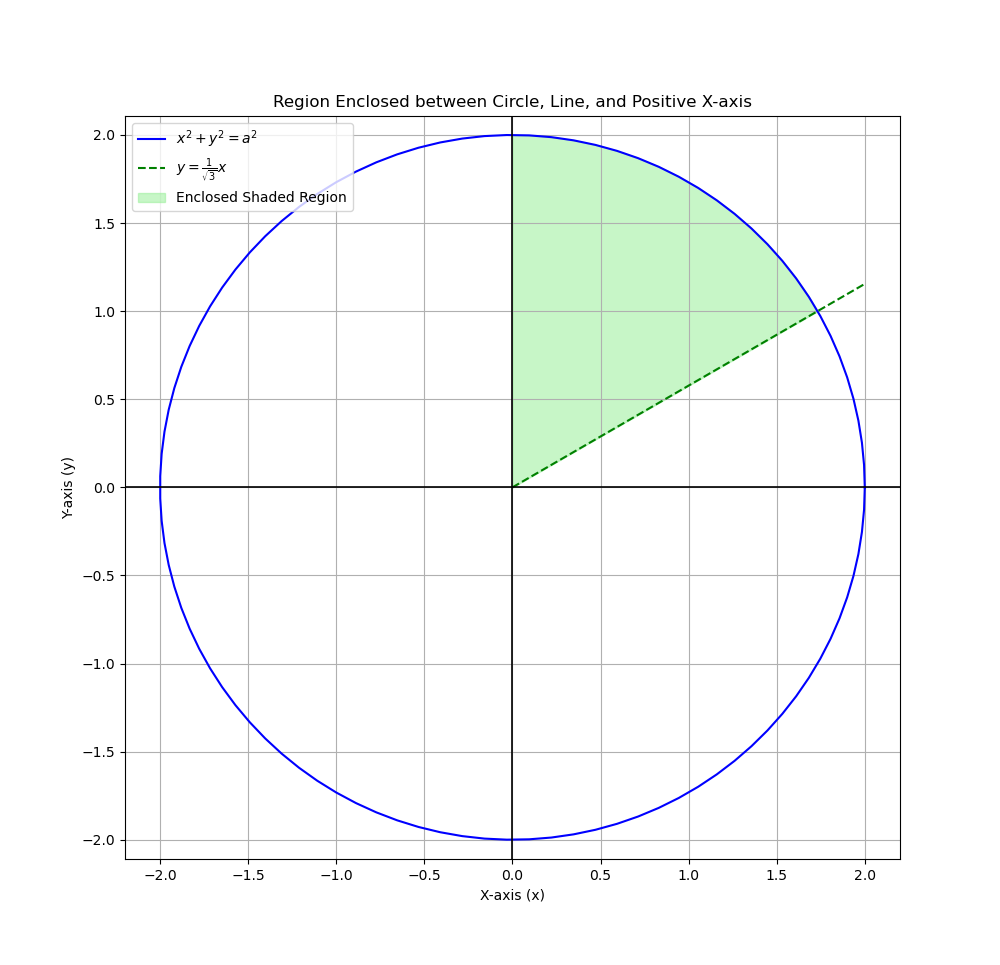
\includegraphics[width=\linewidth]{figs/Figure_1.png}
   \caption{}
   \label{Fig_1}
   \label{stemplot}
\end{figure}





\end{document}
